\documentclass[border=10pt,margin=5pt,tikz,dvisvgm,rgb,utf8]{standalone}
\usepackage{ctex,xeCJK}  % 中文环境
\setCJKmainfont[BoldFont=Source Han Sans SC]{Source Han Serif SC}
\usepackage{calc,fontawesome,forest,smartdiagram,xcolor}
\usetikzlibrary{animations,arrows,automata,graphs,matrix,positioning,shadows,shapes}

\begin{document}
\renewcommand{\baselinestretch}{0.4}

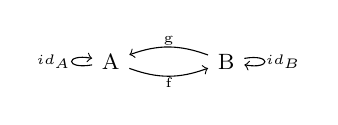
\begin{tikzpicture}
  \node[](A){\footnotesize A};
  \node[right=of A](B){\footnotesize B};

  \path[->]
  (A) edge[out=340,in=200] node[below=-3pt]{\tiny f} (B)
  (A) edge[out=190,in=170, min distance=1em] node[left=-3pt]{\tiny $id_{A}$} (A)
  (B) edge[out=160,in=20] node[above=-3pt]{\tiny g} (A)
  (B) edge[out=10,in=350, min distance=1em] node[right=-3pt]{\tiny $id_{B}$} (B);

\end{tikzpicture}

\end{document}
